%% LectraAI --- IEEE conference-style manuscript
%% Compile with pdflatex (IEEEtran class) + bibtex. Tested structure; if a
%% local TeX install is unavailable, this file compiles unchanged on Overleaf.
%% All numeric values are traceable via ../PAPER_TRACEABILITY.md.
\documentclass[conference]{IEEEtran}
\IEEEoverridecommandlockouts
\usepackage{cite}
\usepackage{amsmath,amssymb,amsfonts}
\usepackage{graphicx}
\usepackage{booktabs}
\usepackage{array}
\usepackage{url}
\usepackage{xcolor}
\usepackage[hidelinks]{hyperref}
\graphicspath{{../figures/}{./figures/}}

\begin{document}

\title{LectraAI: An AI-Assisted Lecture-to-Study-Pack Framework with\\
Duration-Bounded Timestamp Grounding and\\
Deterministic Multi-Format Artifact Transformation}

%% Institution name was not present in the source manuscript and is left as an
%% explicit placeholder (not guessed). Department and city are as supplied.
\author{%
\IEEEauthorblockN{Lakshay Anand}
\IEEEauthorblockA{Information Technology\\
{[Institution name to be completed]}\\
Ghaziabad, India\\
lakshayanand3939@gmail.com\\
Roll No.: 2300320130137}
\and
\IEEEauthorblockN{Harshit Chaudhary}
\IEEEauthorblockA{Information Technology\\
{[Institution name to be completed]}\\
Ghaziabad, India\\
officialharshit111@gmail.com\\
Roll No.: 2300320130113}
\and
\IEEEauthorblockN{Ayush Mavi}
\IEEEauthorblockA{Information Technology\\
{[Institution name to be completed]}\\
Ghaziabad, India\\
ayushmavi2004@gmail.com\\
Roll No.: 2300320130078}
}

\maketitle

%% The primary deliverables (../LECTRAAI_IEEE_RESEARCH_PAPER.pdf / .docx) set the
%% Abstract as a balanced two-column block. Here the standard IEEEtran abstract
%% environment is kept; its text is byte-for-byte identical to those renderings.
\begin{abstract}
Converting long recorded lectures into structured, revision-ready study material is time-consuming, and simple summarization alone does not produce the varied artifacts---organized notes, quizzes, flashcards, revision schedules, interview questions---that learners use when preparing for assessments. This paper presents \textbf{LectraAI}, an end-to-end framework that takes a lecture video, extracts and cleans its transcript, generates structured study notes with a \emph{single} large-language-model (LLM) call constrained by an explicit transcript-grounding prompt, associates generated topics with points in the lecture using a duration-bounded keyword-overlap heuristic, and then produces the remaining study artifacts through \textbf{deterministic (template and regular-expression) transformation of the generated notes} rather than through additional model calls. We describe the implemented system, an instrumented evaluation methodology, and an initial evaluation on \textbf{seven real computer-science lectures}. Within this sample we report: (i) that the timestamp mechanism assigned a topic-level timestamp to 56.0\% of topics (14 of 25), with two of seven lectures receiving none---a coverage characteristic, not a validated accuracy result; (ii) an objective sub-finding on one lecture that the deterministic quiz produced markedly less lexically diverse answer options (44.4\% unique) than a direct-LLM alternative built from the same notes (100\% unique); and (iii) that end-to-end processing latency was strongly and significantly correlated with transcript length (Pearson $r=0.98$, $p<0.001$, $n=7$), with the single LLM call accounting for a mean of 58.7\% of processing time. Human evaluation of timestamp accuracy, artifact quality, and note groundedness was designed and prepared but \textbf{not collected}; consequently three of the four research questions remain inconclusive. We report these limitations explicitly and release the annotation and evaluation infrastructure.
\end{abstract}

\begin{IEEEkeywords}
lecture summarization, educational content generation, large language models, timestamp grounding, deterministic transformation, study-pack generation, transcript processing, reproducible evaluation.
\end{IEEEkeywords}

\section{Introduction}
Recorded lectures are now a primary learning resource, but consuming them for revision is inefficient: a learner must re-watch long videos, pause to take notes, and separately construct practice questions and a revision schedule. Automatic \emph{summarization} of lecture transcripts addresses only part of this workload. Learners preparing for examinations typically rely on several distinct artifact types---organized notes, self-test quizzes, flashcards for spaced recall, a revision timeline, and, in professional contexts, interview-style questions---and they benefit from being able to jump back to the moment in the lecture where a concept was introduced. Producing all of these by hand is laborious, and producing each with a separate LLM call is costly and introduces additional opportunities for ungrounded or inconsistent content.

This paper describes \textbf{LectraAI}, a framework that occupies a specific point in this design space: it uses the LLM once, to generate structured notes under an explicit grounding constraint, and then derives topics, a quiz, flashcards, a revision plan, and interview questions from those notes through \textbf{deterministic transformation} (template filling and regular-expression extraction). Timestamps for generated topics are produced by a lightweight, non-learned heuristic that matches topic keywords against transcript cue markers and validates the result against the video's true duration. The system also renders a printable PDF study pack, persists task state in SQLite, and instruments each processing stage for measurement.

We frame the investigation around four research questions, whose evidence status is drawn from the project's internal audit:
\begin{itemize}
\item \textbf{RQ1---Timestamp grounding:} How accurately does LectraAI's timestamp mechanism associate generated study content with relevant points in the lecture?
\item \textbf{RQ2---Artifact generation strategy:} How does LectraAI's deterministic artifact transformation compare with direct LLM-generated educational artifacts in terms of artifact quality?
\item \textbf{RQ3---Prompt ablation / groundedness:} How do explicit grounding constraints in the LectraAI prompt affect the groundedness of generated notes relative to an unconstrained prompt?
\item \textbf{RQ4---Processing efficiency:} How does lecture/transcript length relate to end-to-end processing latency?
\end{itemize}

\noindent\textbf{Contributions.} We classify our contributions conservatively:
\begin{enumerate}
\item \emph{(System / engineering)} An end-to-end, instrumented lecture-to-study-pack architecture combining dual-strategy transcript extraction, single-call grounded note generation, a duration-bounded timestamp-association heuristic, deterministic multi-format artifact transformation, PDF assembly, and task persistence with graceful model fallback.
\item \emph{(System / methodological)} A duration-bounded timestamp-association mechanism that constrains topic--time associations using the video's true duration and embedded transcript cue markers, with a reproducible protocol for evaluating its \emph{coverage} and its \emph{divergence from a naive baseline} in the absence of human ground truth.
\item \emph{(Methodological)} An experimental framework---with released baselines and materials---for comparing (a) deterministic artifact transformation against direct-LLM artifact generation from identical notes, and (b) grounded against unconstrained prompting, holding the transcript and model fixed.
\item \emph{(Empirical, evaluated-sample only)} An analysis of end-to-end processing latency with respect to transcript length on seven real lectures, including a per-stage breakdown.
\end{enumerate}
We do \emph{not} claim that LectraAI produces accurate timestamps, higher-quality artifacts than an LLM baseline, or reduced hallucination; the evidence required for those claims (human annotation and rating) was not collected.

\section{Related Work}
\textbf{Lecture and educational-video summarization.} Deep-learning approaches to video summarization are surveyed by Apostolidis \emph{et al.}~\cite{apostolidis2021}. Lecture-specific note generation from slide-based videos was demonstrated by Xu \emph{et al.}~\cite{xu2019}, and multimodal lecture understanding has a dedicated benchmark from Lee \emph{et al.}~\cite{lee2023}. Transcript quality is an upstream variable: Kuhn \emph{et al.}~\cite{kuhn2023} measure commercial ASR accuracy on higher-education lectures and find wide vendor variation. LectraAI consumes platform-provided captions rather than performing its own speech recognition, and operates on transcript text only.

\textbf{LLM-based educational content generation.} Broad reviews of LLMs in learning environments discuss personalization, adaptability, and factual-reliability concerns~\cite{shahzad2025}. Lin \emph{et al.}~\cite{lin2025} report that decomposing generation into sub-tasks improves human-rated lesson quality relative to single-step generation---relevant to LectraAI's single-call design, which trades that potential gain for cost and consistency.

\textbf{Automatic question and distractor generation.} Educational question generation with LLMs, including Bloom's-taxonomy alignment, is studied by Scaria \emph{et al.}~\cite{scaria2024}, with methodology-and-educator-insight work by Biancini \emph{et al.}~\cite{biancini2024}. Distractor generation is surveyed by Alhazmi \emph{et al.}~\cite{alhazmi2024}; neural distractor generation predates the LLM era~\cite{qiu2020}, and preprint work explores fine-tuned question generation~\cite{ehsan2025}. A consistent theme is that automated evaluation does not substitute for human judgement of question quality. LectraAI's quiz is produced by fixed templates rather than by a model.

\textbf{Flashcards and spaced repetition.} Sentence generation for spaced-repetition practice has been evaluated with real learners by Paddags \emph{et al.}~\cite{paddags2024}, and retrieval-augmented generation of such content by Kaczmarek \emph{et al.}~\cite{kaczmarek2025}. Optimal, learner-adaptive review scheduling is established by Tabibian \emph{et al.}~\cite{tabibian2019}. LectraAI's flashcards are extracted verbatim from the generated notes, and its revision plan is a fixed schedule with no learner-performance input.

\textbf{Temporal grounding.} Associating natural-language content with points in a video has two recent surveys~\cite{zhang2023,liu2023}; state-of-the-art methods are learned and multimodal. LectraAI's timestamp mechanism is deliberately simpler---text-only keyword overlap against transcript cue markers, bounded by video duration---and is evaluated here only on coverage and divergence.

\textbf{Hallucination and grounding.} Hallucination in LLMs is surveyed by Huang \emph{et al.}~\cite{huang2023}, with education-specific risk discussion by Peltekova \emph{et al.}~\cite{peltekova2026}; mitigation in the literature is dominated by retrieval augmentation and fine-tuning. LectraAI instead uses prompt-only negative constraints, which our RQ3 was designed to ablate.

\textbf{Integrated systems.} The closest prior integrated system is NoteIt~\cite{zhao2025}, which converts instructional videos into interactive notes through multimodal understanding and was user-tested. LectraAI differs in being transcript-only and producing several distinct artifact types; the combination of artifact types is not claimed as a novelty in itself.

\section{The LectraAI Framework}
\subsection{Overview}
Fig.~\ref{fig:arch} shows the implemented pipeline. A lecture URL is submitted; the backend creates an asynchronous task, extracts and cleans the transcript, issues \emph{one} grounded LLM call to generate Markdown study notes, applies regular-expression clean-up, and then performs \textbf{deterministic transformation} of the notes into: segmented topics, topic timestamps, a multiple-choice quiz, flashcards, a five-stage revision plan, and tiered interview questions. The study pack is serialized to JSON, rendered to a PDF, and the task's terminal state plus per-stage instrumentation are stored in SQLite.

\textbf{Critical distinction.} Only the note-generation stage is model-generated. Topics, timestamps, quiz, flashcards, revision plan, and interview questions are produced by template and regular-expression logic operating on the generated notes; no further model call is made. We describe the system as \emph{AI-assisted study-pack generation followed by deterministic multi-format transformation}, and avoid the phrasing ``AI-generated'' for the derived artifacts.

\begin{figure*}[t]
\centering
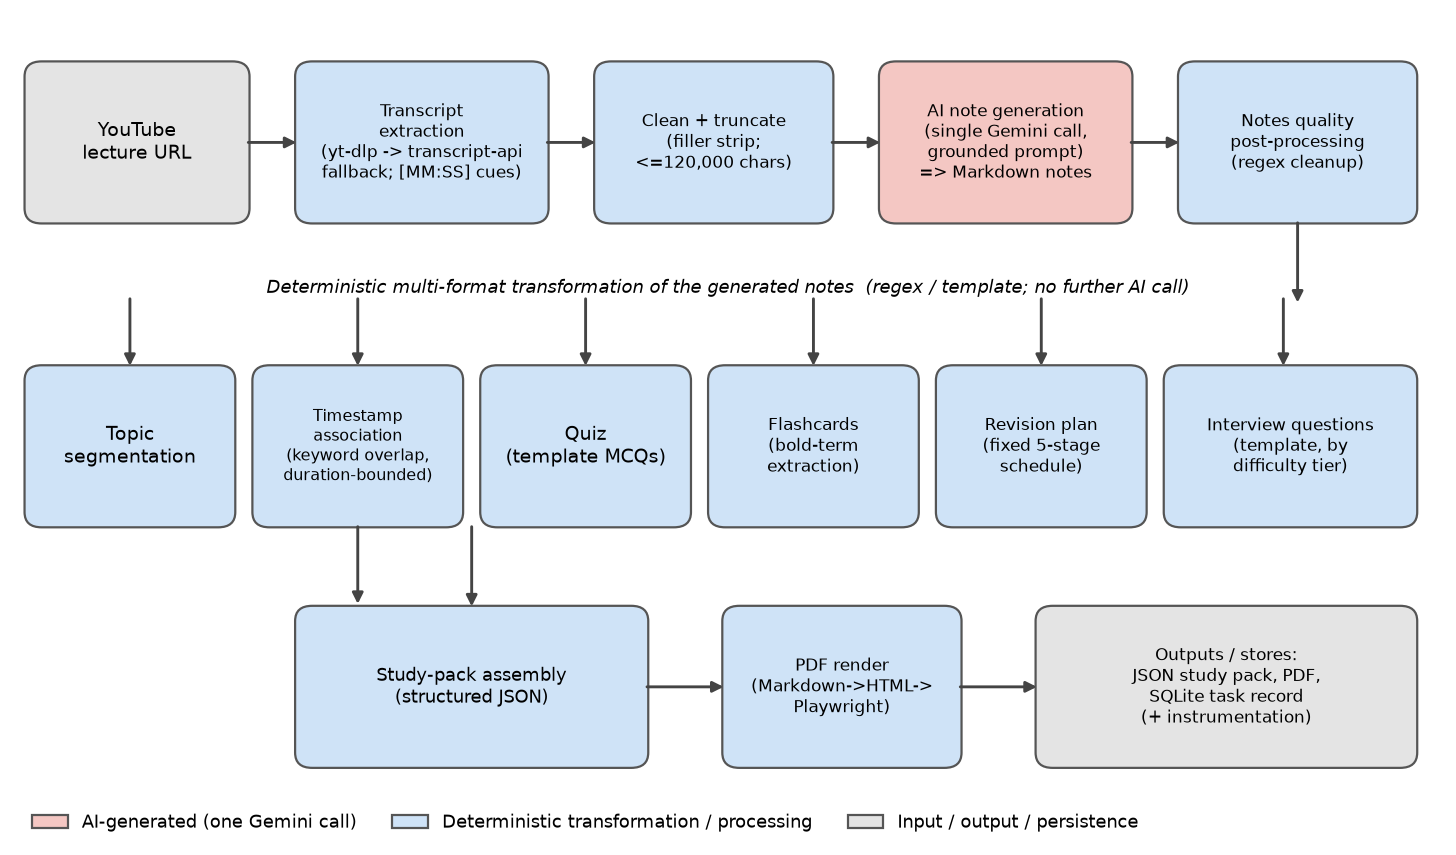
\includegraphics[width=0.94\textwidth]{fig0_architecture.png}
\caption{LectraAI pipeline architecture (schematic of the verified implementation). Pink: the single AI-generated stage (one Gemini call). Blue: deterministic transformation and processing. Grey: input, output, and persistence. Derived artifacts are transformations of the generated notes, not independent model outputs.}
\label{fig:arch}
\end{figure*}

\subsection{Transcript acquisition and cleaning}
The transcript is obtained by a dual-strategy fetcher: first via a subtitle-download path (\texttt{yt-dlp} with optional authenticated cookies), then, on failure, via a transcript API. Retrieved captions are concatenated with an inserted \texttt{[MM:SS]} (or \texttt{[H:MM:SS]} past one hour) \textbf{cue marker} whenever a gap of at least 60~s occurs between consecutive caption segments; the video duration is captured from the fetch metadata. The transcript is de-duplicated, stripped of common spoken-filler and channel-promotional phrases via regular expressions, and truncated to a maximum of $120{,}000$ characters before the model call. In the evaluated dataset the longest transcript was $59{,}821$ characters, so truncation never triggered.

\subsection{Grounded note generation}
A single call is made with a prompt (\texttt{SMART\_PROMPT\_v1}) containing an explicit block of \textbf{strict negative constraints}: write only content traceable to the transcript; do not complete the lecture with outside knowledge; do not invent examples or analogies; preserve the lecturer's claim strength. The model returns one Markdown document. A subsequent regular-expression pass removes residual transcript intros, generic section titles, and internal identifiers, and softens a small set of over-strong phrasings. If every model/API attempt fails, a local non-model heuristic note generator is used; the evaluated runs did not trigger this path.

\subsection{Deterministic transformation}
From the generated notes: \textbf{topics} come from splitting on level-two headings (title, text, up to six bullet key points, optional diagram block); \textbf{timestamps} from Section~\ref{sec:ts}; \textbf{quiz} items from fixed question templates per topic with incorrect options drawn from a small fixed pool of generic sentences, then correct-option position shuffled; \textbf{flashcards} by pairing each extracted bold term with its containing sentence; \textbf{revision plan} as a fixed five-stage schedule (24~h, 3~d, 7~d, 14~d, 30~d) with only the per-stage topic-title list varying; \textbf{interview questions} from fixed templates assigned round-robin to difficulty tiers by topic index.

\subsection{Assembly, rendering, persistence}
Artifacts are assembled into one JSON study pack (also exposing the raw notes, video duration, and grounded timestamp list). Notes are converted Markdown$\rightarrow$HTML and rendered to an A4 PDF by a headless-browser subprocess. Task lifecycle (\texttt{pending}$\rightarrow$\texttt{processing}$\rightarrow$\texttt{completed}$\,|\,$\texttt{failed}) is persisted in SQLite; a startup routine marks any task left in \texttt{processing} as \texttt{failed}. Repeat submissions are served from a file cache keyed by video identifier unless a forced refresh is requested.

\subsection{Research instrumentation}
For measurement, the task record additionally stores the generation method (model vs.\ offline fallback), the model that responded, the prompt version, and the transcript character count; a separate table stores start/end timestamps for the transcript-fetch, AI-generation, transformation, and PDF-render stages. This instrumentation is additive and does not alter processing behaviour (the system's test suite passes unchanged with it enabled).

\section{Methodology}
We separate the \textbf{production system} (Section~III) from \textbf{research-only components} (baselines and evaluation scripts used only for this study, never invoked by the deployed pipeline).

\subsection{Lecture acquisition}
Lectures were selected as publicly accessible computer-science lectures with usable captions, an identifiable duration, and coherent content. Each was processed once through the unmodified production pipeline with a forced refresh so all instrumentation fields were populated by a genuine run.

\subsection{Duration-bounded timestamp association}\label{sec:ts}
For a topic with title $t$ and video duration $D$: (i) if the topic text contains an explicit cue at second $s$ with $0 \le s < D$, assign it; otherwise (ii) extract search terms from the cleaned title, score each transcript cue by the number of search terms present in its text (with a small bonus for domain acronyms), and assign the highest-scoring cue with $0 \le s < D$ provided its score is at least~1. Topics for which no cue clears the threshold receive \emph{no} topic-level timestamp. The final list is sorted chronologically and entries with $s \ge D$ discarded.

Two quantities are computed without human ground truth. \textbf{Topic--timestamp coverage} is the fraction of generated topics that received a timestamp. \textbf{Divergence from a naive baseline} is, for timestamped topics, the mean of the per-topic absolute error
\begin{equation}
e_i \;=\; \bigl|\, \hat{s}_i - b_i \,\bigr|, \qquad
b_i \;=\; \frac{i\,D}{n},
\label{eq:div}
\end{equation}
where $\hat{s}_i$ is the assigned second for topic $i$ of $n$ and $b_i$ is the naive equal-interval position. Both quantities are descriptive; neither is an accuracy measure.

\subsection{Research-only baselines}
\emph{(1) Naive equal-interval timestamps}~\eqref{eq:div}, the null comparison for RQ1. \emph{(2) Direct-LLM artifact generator:} given the \emph{same} generated notes, one model call per artifact type requesting the same JSON structure; the comparison condition for RQ2; \emph{not} part of LectraAI. \emph{(3) Unconstrained note prompt:} \texttt{SMART\_PROMPT\_v1} with only the constraint block removed, everything else identical; programmatically verified to differ only in that block; the comparison condition for RQ3. An extractive TF--IDF summarization baseline was implemented but \textbf{excluded} after a real-transcript trial showed spoken-lecture transcripts collapse its sentence segmentation.

\subsection{Metrics and their evidence requirements}
\textbf{Timestamp accuracy (RQ1):} $|\,t_{\text{pred}} - t_{\text{ref}}\,|$ against a human reference window, aggregated as MAE, median absolute error, and percentage within $\pm5/10/30$~s. \emph{Requires human reference timestamps; not computed.} A tolerance-window protocol and per-lecture annotation packages were prepared for all seven lectures.
\textbf{Artifact quality (RQ2):} blinded human ratings (correctness, relevance, coverage, distractor plausibility, difficulty; 1--5). \emph{Not collected.} Two objective structural metrics were computed instead---\textbf{distractor uniqueness} (unique distractor strings $\div$ total) and \textbf{flashcard verbatim overlap} (answers found verbatim in notes $\div$ total)---and are labelled as diversity/behaviour, not quality.
\textbf{Groundedness (RQ3):} human claim-level classification against the transcript, aggregated as an unsupported-claim rate. \emph{Not collected.} An automated proxy was attempted and \textbf{excluded} for construct-invalidity (miscounting Markdown headers as claims; missing orthographic variants). A mechanical claim-segmentation (58 units) was prepared for a future human pass.
\textbf{Latency (RQ4):} per-stage and total wall-clock time from instrumentation; its relationship to transcript length via the Pearson correlation. \emph{Requires no human judgement; computed.}

\subsection{Statistical analysis}
Descriptive statistics are reported for all quantities. For RQ4, the Pearson correlation between transcript character count and total latency is reported with its two-sided $p$-value at $n=7$. No inferential test is applied to RQ1--RQ3: RQ1 has no ground truth, and RQ2/RQ3 have single-lecture data. All previously reported values were independently recalculated from raw data during the project's audit (9 of 9 confirmed; one aggregation-convention ambiguity disclosed in Section~\ref{sec:rq4}).

\section{Experimental Setup}
\subsection{Dataset}
The evaluated dataset consists of \textbf{$N=7$ real computer-science lectures} (Table~\ref{tab:dataset}). All seven were processed successfully via a genuine model call (0 offline-fallback invocations, 0 failures); the responding model was recorded as \texttt{gemini-3.6-flash} for every run, under prompt version \texttt{SMART\_PROMPT\_v1}. The dataset is small, skewed toward short lectures, contains no coding-implementation or numerical lecture, and represents four subject domains. A dataset-expansion attempt did not yield additional individually-verifiable lecture identifiers with the available tooling.

\begin{table}[t]
\caption{Dataset characteristics ($N=7$).}
\label{tab:dataset}
\centering
\begin{tabular}{@{}p{0.44\columnwidth}p{0.46\columnwidth}@{}}
\toprule
\textbf{Property} & \textbf{Value} \\
\midrule
Lectures & 7 \\
Duration (s): mean / median & 1163.9 / 777.0 \\
\quad min / max / SD & 393.0 / 3702.3 / 1140.9 \\
Duration bands & Short ($\le$15\,min): 5; Medium: 1; Long ($>$45\,min): 1 \\
Transcript length (chars): mean / median & 17{,}109 / 10{,}590 \\
\quad min / max / SD & 5{,}326 / 59{,}821 / 19{,}006 \\
Subject domains & OS: 2; Networks: 2; DBMS: 2; AI: 1 \\
Lecture-type categories & Comparison: 3; Architecture: 2; Algorithm: 1; Theory: 1 \\
Caption source recorded & 0 of 7 \\
Language & English (all 7) \\
\bottomrule
\end{tabular}
\end{table}

\subsection{Human evaluation status}
Human timestamp annotations: \textbf{0}. Human artifact ratings: \textbf{0}. Human claim-level groundedness labels: \textbf{0}. The corresponding infrastructure (protocols, schemas, per-lecture packages, rubrics, blinding procedure) is complete and released; only the human-collected data is absent.

\subsection{Reproducibility notes}
The implementation documentation names a different model identifier (\texttt{gemini-2.5-flash}) than the code's fallback list; the instrumentation recorded \texttt{gemini-3.6-flash} as the responder for all seven runs, and that value is authoritative here. Sampling parameters (temperature, top-$p$) are not set in the code and not independently recorded---an acknowledged reproducibility limitation. All raw/processed result files, the seven study-pack JSON outputs, the figures, and the analysis scripts are in the project repository.

\section{Results}
\subsection{RQ1---Timestamp grounding (INCONCLUSIVE)}
Across the seven lectures the pipeline generated \textbf{25 topics}; the timestamp mechanism assigned a topic-level timestamp to \textbf{14 (56.0\% coverage)}. \textbf{Two lectures} received \emph{no} topic-level timestamps at all. For the 14 timestamped topics, the assigned times diverged from the naive equal-interval baseline by a \textbf{mean of 147.3~s} (median 124.0~s, SD 93.0~s; Table~\ref{tab:rq1}). Fig.~\ref{fig:cov} shows per-lecture coverage.

\begin{table}[t]
\caption{RQ1---timestamp coverage and divergence from the naive baseline.}
\label{tab:rq1}
\centering
\begin{tabular}{@{}lccc@{}}
\toprule
\textbf{Lecture} & \textbf{Topics} & \textbf{With timestamp} & \textbf{Mean $|\Delta|$ vs.\ naive (s)} \\
\midrule
3MqyDWDpZoI & 5 & 3 & 150.2 \\
1msEo8PIcbw & 3 & 0 & --- \\
T4lGm7MjA6Y & 5 & 0 & --- \\
uDulBxDb7GM & 3 & 2 & 168.5 \\
VyvTabQHevw & 2 & 2 & 101.3 \\
WJ-UaAaumNA & 5 & 5 & 143.5 \\
ZtVw2iuFI2w & 2 & 2 & 177.0 \\
\midrule
\textbf{Total / mean} & \textbf{25} & \textbf{14 (56.0\%)} & \textbf{147.3 ($n{=}14$)} \\
\bottomrule
\end{tabular}
\end{table}

\noindent\textbf{Interpretation.} Coverage of 56\% is an \textbf{output characteristic of the mechanism, not a validated accuracy measure}; without human reference timestamps we cannot say whether the assigned times are correct, and large divergence from the naive baseline could indicate either better or worse localization. RQ1 is \textbf{inconclusive}.

\begin{figure}[t]
\centering
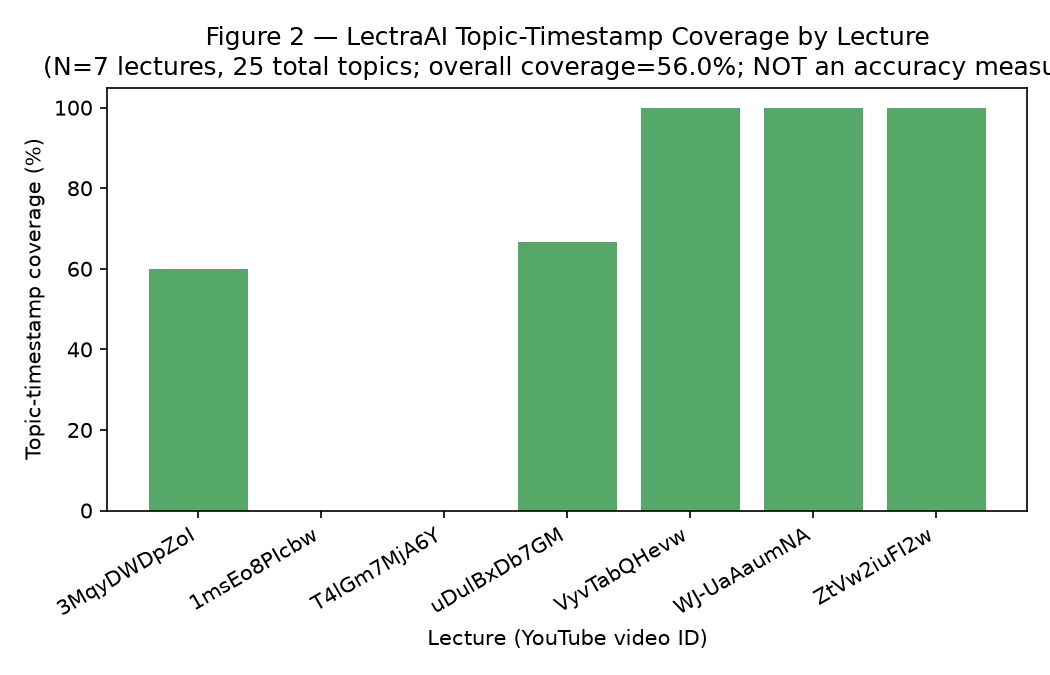
\includegraphics[width=0.98\columnwidth]{fig2_topic_timestamp_coverage.png}
\caption{LectraAI topic--timestamp coverage by lecture ($N=7$, 25 topics). Not an accuracy measure. Two lectures have zero topic-level coverage.}
\label{fig:cov}
\end{figure}

\subsection{RQ2---Artifact generation strategy (INCONCLUSIVE; one narrow diversity sub-finding)}
Direct-LLM comparison artifacts were generated from the notes of \textbf{one lecture} (\texttt{3MqyDWDpZoI}), using the same model and source notes as the production pipeline. Two objective structural metrics were computed (Table~\ref{tab:rq2}, Fig.~\ref{fig:distract}).

\begin{table}[t]
\caption{RQ2---objective structural metrics (one lecture, \texttt{3MqyDWDpZoI}).}
\label{tab:rq2}
\centering
\begin{tabular}{@{}p{0.40\columnwidth}cc@{}}
\toprule
\textbf{Metric} & \textbf{LectraAI (det.)} & \textbf{Direct-LLM} \\
\midrule
Quiz distractor uniqueness & 8/18 (44.4\%) & 27/27 (100.0\%) \\
Flashcard answer verbatim in notes & 10/10 (100.0\%) & 1/9 (11.1\%) \\
\bottomrule
\end{tabular}
\end{table}

\noindent\textbf{Interpretation.} The distractor-diversity difference is a \textbf{real, objective, single-lecture} observation consistent with the design (fixed templates vs.\ content-specific generation). It is a \textbf{diversity} result, not a quality result: a diverse distractor may still be wrong, and a repeated-template distractor may still be a valid incorrect option. \textbf{Overall artifact-quality superiority of either approach was not established}---no human ratings exist for any artifact type, and only one lecture was compared. RQ2 is \textbf{inconclusive}, with one narrow supported sub-finding on distractor diversity.

\begin{figure}[t]
\centering
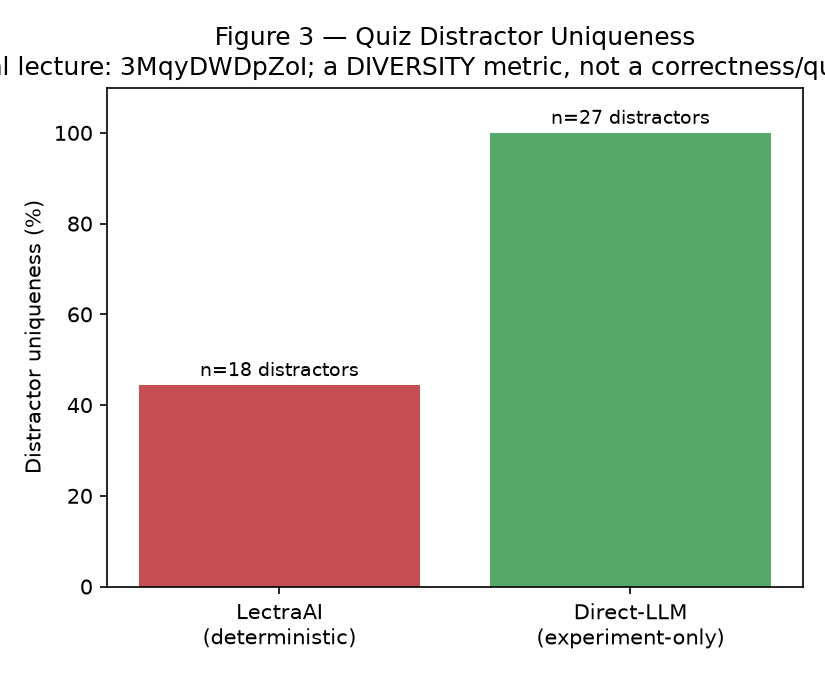
\includegraphics[width=0.80\columnwidth]{fig3_distractor_uniqueness.png}
\caption{Quiz distractor uniqueness for one lecture. A diversity metric, not a correctness or quality rating.}
\label{fig:distract}
\end{figure}

\subsection{RQ3---Prompt ablation / groundedness (INCONCLUSIVE)}
Notes were generated for one lecture under both the constrained production prompt and the unconstrained prompt, from the identical transcript and model; the prompts were verified to differ only in the removed constraint block (constrained notes: 3{,}890 characters; unconstrained: 3{,}763). An automated groundedness proxy was attempted and \textbf{excluded} for construct-invalidity. \textbf{No human claim-level groundedness labels were collected.} RQ3 is \textbf{inconclusive because human ground truth was not collected}; a mechanical claim-segmentation (58 units) has been prepared for a future human pass.

\subsection{RQ4---Processing efficiency (SUPPORTED for the evaluated sample)}\label{sec:rq4}
Per-lecture and aggregate latency are in Table~\ref{tab:rq4}. Total end-to-end latency had a \textbf{mean of 39.2~s} (median 34.2~s, SD 12.2~s, range 32.0--66.3~s). The single AI-generation call was the dominant stage in every case, at a mean of \textbf{58.7\%} of total latency per lecture (an alternative aggregation---the ratio of the two means---gives 59.9\%; both are reported). The deterministic transformation stage was negligible (mean 0.05~s). There were \textbf{0 model-fallback invocations and 0 failures}.

\begin{table}[t]
\caption{RQ4---per-lecture processing latency (seconds).}
\label{tab:rq4}
\centering
\setlength{\tabcolsep}{3.2pt}
\begin{tabular}{@{}lcccccc@{}}
\toprule
\textbf{Lecture} & \textbf{Chars} & \textbf{Fetch} & \textbf{AI gen.} & \textbf{Transf.} & \textbf{PDF} & \textbf{Total} \\
\midrule
uDulBxDb7GM & 8{,}556 & 9.39 & 17.13 & 0.03 & 5.04 & 31.98 \\
ZtVw2iuFI2w & 10{,}424 & 5.08 & 19.02 & 0.11 & 7.92 & 32.41 \\
VyvTabQHevw & 11{,}553 & 9.15 & 19.37 & 0.04 & 4.52 & 33.27 \\
3MqyDWDpZoI & 5{,}326 & 9.99 & 19.06 & 0.04 & 4.78 & 34.25 \\
WJ-UaAaumNA & 13{,}495 & 9.01 & 24.25 & 0.04 & 4.52 & 38.01 \\
1msEo8PIcbw & 10{,}590 & 13.28 & 19.89 & 0.03 & 4.86 & 38.21 \\
T4lGm7MjA6Y & 59{,}821 & 14.90 & 45.73 & 0.09 & 5.46 & 66.34 \\
\midrule
\textbf{Mean} & \textbf{17{,}109} & \textbf{10.12} & \textbf{23.49} & \textbf{0.05} & \textbf{5.30} & \textbf{39.21} \\
\bottomrule
\end{tabular}
\end{table}

The Pearson correlation between transcript character count and total latency was $r = 0.98$ ($p \approx 8.9\times10^{-5}$, i.e.\ $p < 0.001$; $n = 7$). Fig.~\ref{fig:latvs} plots the relationship; Fig.~\ref{fig:latstage} shows the per-stage breakdown.

\begin{figure}[t]
\centering
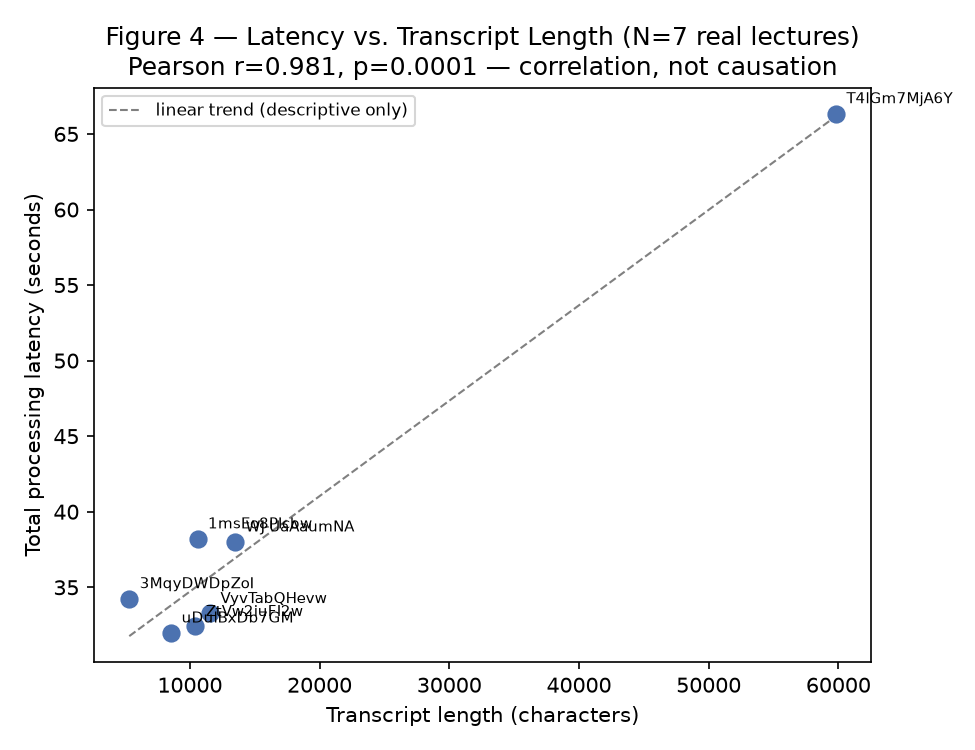
\includegraphics[width=0.98\columnwidth]{fig4_latency_vs_transcript_length.png}
\caption{End-to-end latency vs.\ transcript length ($N=7$; Pearson $r=0.98$, $p<0.001$). Correlation, not causation; the dashed line is a descriptive trend only.}
\label{fig:latvs}
\end{figure}

\begin{figure}[t]
\centering
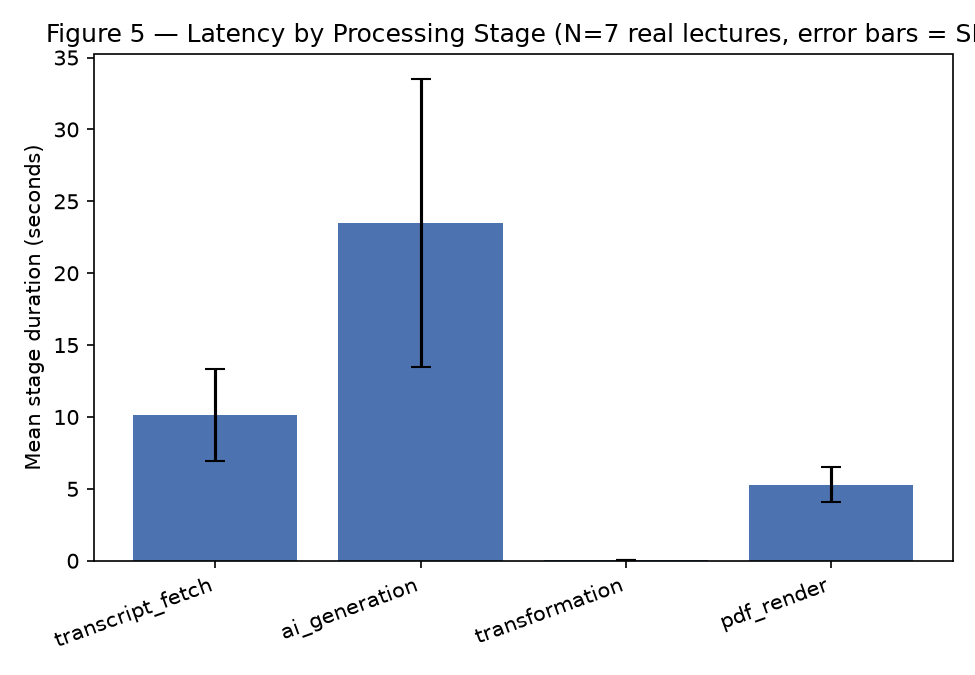
\includegraphics[width=0.98\columnwidth]{fig5_latency_stage_breakdown.png}
\caption{Latency by processing stage ($N=7$; error bars = SD). The single model call dominates.}
\label{fig:latstage}
\end{figure}

\noindent\textbf{Interpretation.} Within this seven-lecture sample, transcript length shows a strong, statistically significant positive association with end-to-end latency, and processing time is dominated by the single model call. This is a \textbf{correlation}, not a causal relationship, and it is \textbf{specific to this sample and this measurement window}: latency includes network-dependent components that vary over time, and the sample spans only three duration bands with a single lecture above 20~minutes. We do not claim linear or universal scaling.

\subsection{Result validation}
All nine quantitative results reported earlier in the project were independently recalculated from raw data and confirmed. The only noted discrepancy is definitional: the AI-stage latency share can be aggregated as a per-lecture mean of ratios (58.7\%) or a ratio of means (59.9\%); we report both.

\section{Discussion}
\textbf{What the evidence supports.} Two claims are defensible. First, the timestamp mechanism has \textbf{incomplete coverage}---56\% of topics overall, 0\% for two of seven lectures---independent of any accuracy question: the mechanism sometimes produces nothing to evaluate. The likely cause is the keyword-overlap score's minimum threshold combined with terse, acronym-heavy topic titles and sparse cue text. Second, within the evaluated sample, \textbf{latency scales with transcript length and is dominated by the model call}; the practical implication is that the model call is the component to optimize or budget for.

\textbf{What the evidence does not support.} We cannot conclude anything about timestamp \emph{accuracy}, about artifact \emph{quality} relative to an LLM baseline, or about \emph{hallucination} reduction. The distractor-diversity result shows a real structural consequence of the template approach, but structural diversity is necessary, not sufficient, for good distractors, and the result is from a single lecture.

\textbf{Design implications.} The single-call-plus-deterministic-transformation architecture has a measured cost profile ($\sim$0.05~s derivation) and a measured structural limitation (low distractor diversity). Whether that trade-off is acceptable depends on a quality measurement not yet made; the literature~\cite{lin2025,scaria2024,alhazmi2024,qiu2020} suggests model-based generation tends to produce higher-rated educational questions, motivating the RQ2 human study.

\textbf{Positioning.} Relative to NoteIt~\cite{zhao2025} and prior lecture-note systems~\cite{lee2023,xu2019}, LectraAI is transcript-only and multi-artifact; it does not use a visual channel and, on current evidence, makes no quality claim. Its timestamp mechanism is far simpler than learned temporal grounding~\cite{zhang2023,liu2023}.

\section{Limitations}
(1) Small dataset ($N=7$). (2) Limited domain/format diversity---no coding or numerical lecture; five of seven under 15~minutes. (3) No human timestamp ground truth (RQ1 accuracy unevaluated). (4) No human artifact ratings (RQ2 quality unevaluated; one lecture only). (5) No human groundedness labels (RQ3 unevaluated; automated proxy rejected). (6) Excluded extractive baseline (transcript-format incompatibility). (7) Model configuration variability---sampling parameters unpinned; documentation/code disagree on the model identifier. (8) Single measurement window for RQ4. (9) No generalization claim beyond the seven-lecture sample. (10) No comparison with third-party systems. (11) Tooling limitation for dataset growth. (12) No OCR/multimodal input and no user study, by design.

\section{Future Work}
Infrastructure is prepared and released for: collecting human timestamp annotations and computing MAE / median error / $\pm5/10/30$~s accuracy (RQ1); the blinded human artifact evaluation across multiple lectures (RQ2); claim-level groundedness labelling for the two prompt conditions (RQ3); dataset expansion to 18--20 lectures with coding/numerical coverage; pinning and recording model sampling parameters; investigating the timestamp coverage-failure mode and evaluating stronger alignment methods; and broadening the RQ4 measurement across sessions and to longer lectures.

\section{Conclusion}
We presented LectraAI, an instrumented, end-to-end framework that turns a lecture video into a structured study pack using a single grounded LLM call for the notes and deterministic transformation for the remaining artifacts, with a duration-bounded heuristic for topic timestamps. On seven real computer-science lectures we found that the timestamp mechanism covers 56\% of topics (two lectures at 0\%), that the deterministic quiz is markedly less lexically diverse than a direct-LLM alternative on the one lecture compared, and that end-to-end latency is strongly correlated with transcript length and dominated by the model call. Human evaluation of timestamp accuracy, artifact quality, and groundedness was designed and prepared but not collected, so three of four research questions remain inconclusive. We release the full evaluation infrastructure and identify the specific human studies needed to complete the assessment.

\bibliographystyle{IEEEtran}
\bibliography{references}

\end{document}
